\subsubsection{June 12}

\subsubsection*{True (\trueIcon) false (\falseIcon) questions}

\begin{enumerate}
    \item \trueIcon \: Virtualization can reduce costs by enabling the sharing of hardware resources between virtual machines.
    \item \trueIcon \: In-row cooling systems allow for higher server densities and increased rack power densities in datacenters.
    \item \falseIcon \: RAID 6 offers better random and sequential write performance than RAID 5.
    \item \trueIcon \: The computing continuum refers to the idea that computing devices exist on a spectrum, from small, low-power devices to large, high-performance machines.
    \item \trueIcon \: In-row cooling involves placing cooling units between server racks.
    \item \falseIcon \: Full virtualization can run on a wider range of hardware than paravirtualization.
    \item \falseIcon \: In current datacenters east-west traffic typically involves lower data volumes compared to north-south traffic.
    \item \trueIcon \: TPUs are more power-efficient and offer higher performance compared to GPUs in deep learning tasks.
    \item \falseIcon \: DAS devices connect directly to a network and are accessed over the network by clients.
    \item \trueIcon \: Controlling humidity levels in a datacenter is important for preventing equipment failures.
\end{enumerate}

\newpage

\subsubsection*{Exercises}

\begin{enumerate}
    \setcounter{enumi}{10}
    \item Suppose we have a computer system composed of 6 different components, and designed to have an RBD as shown in the image below. The four types of components (A, B, C, and D) have different reliability characteristics. We know that after 2 years the reliability of components B, C, and D are respectively $R_B(2y) = 0.8$, $R_C(2y) = 0.6$, and $R_D(2y) = 0.9$. What should be the MTTF for component A, if we want to have a Reliability of the whole system after 2 years equal to $R_{sys}(2y) = 0.82$? Use always at least 3 decimal digits for each calculation.
    
    \begin{center}
        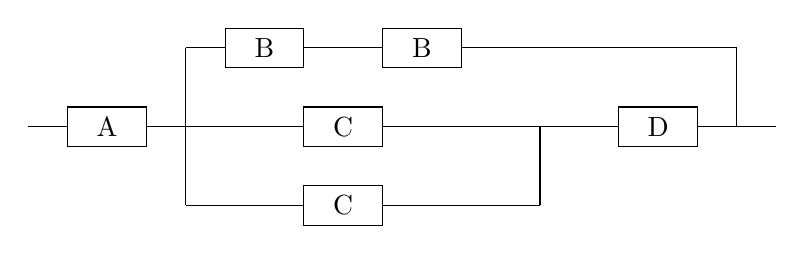
\begin{tikzpicture}[node distance=1cm]
            \node[
                draw,
                minimum width=1cm,
                minimum height=0.5cm,
                name=A
            ] at (1,0) {A};
            \node[
                draw,
                minimum width=1cm,
                minimum height=0.5cm,
                name=B1
            ] at (3,1) {B};
            \node[
                draw,
                minimum width=1cm,
                minimum height=0.5cm,
                name=B2
            ] at (5,1) {B};
            \node[
                draw,
                minimum width=1cm,
                minimum height=0.5cm,
                name=C1
            ] at (4,0) {C};
            \node[
                draw,
                minimum width=1cm,
                minimum height=0.5cm,
                name=C2
            ] at (4,-1) {C};
            \node[
                draw,
                minimum width=1cm,
                minimum height=0.5cm,
                name=D
            ] at (8,0) {D};

            \draw (0,0) -- (A);
            \draw (A) -- (2,0);
            
            \draw (2,0) -- (2,1);
            \draw (2,0) -- (C1);
            \draw (2,0) -- (2,-1);

            \draw (2,1) -- (B1);
            \draw (B1) -- (B2);
            \draw (2,-1) -- (C2);

            \draw (C1) -- (6.5,0);
            \draw (C2) -- (6.5,-1);
            \draw (6.5,-1) -- (6.5,0);
            \draw (6.5,0) -- (D);

            \draw (B2) -- (9,1);
            \draw (9,1) -- (9,0);
            \draw (D) -- (9.5,0);
        \end{tikzpicture}
    \end{center}

    \textcolor{Green3}{\textbf{\emph{Answer:}}} We have 4 groups here:
    \begin{enumerate}[label=Group \arabic*., labelwidth=4em, labelsep=1em, leftmargin=!]
        \item The two C components are \textbf{parallel}. The reliability of C is $0.6$, so:
        \begin{equation*}
            \begin{array}{rcl}
                R_{\text{Group 1}} &=& 1 - \displaystyle\prod_{i=1}^{n=2} \left(1 - R_{C_i}\right) \\ [1.5em]
                &=& 1 - \left[
                    \left(1 - 0.6\right)
                    \cdot
                    \left(1 - 0.6\right)
                \right] \\ [.5em]
                &=& 1 - 0.16 \\ [.5em]
                &=& 0.84
            \end{array}
        \end{equation*}
        \item Group 1 and component D are \textbf{sequential}. The reliability of D is $0.9$, and the reliability of group 1 is $0.84$, so:
        \begin{equation*}
            R_{\text{Group 2}} = \displaystyle\prod_{i=1}^{n=2} R_{i} = 0.9 \cdot 0.84 = 0.756
        \end{equation*}
        \item The two B components are \textbf{sequential}. The reliability of B is $0.8$, so:
        \begin{equation*}
            R_{\text{Group 3}} = \displaystyle\prod_{i=1}^{n=2} R_{B_i} = 0.8 \cdot 0.8 = 0.64
        \end{equation*}
        \item Groups 3 and 2 are \textbf{parallel}. The reliability of the group 2 is $0.756$ and the reliability of the group 3 is $0.64$, so:
        \begin{equation*}
            \begin{array}{rcl}
                R_{\text{Group 4}} &=& 1 - \displaystyle\prod_{i=1}^{n=2} \left(1 - R_{i}\right) \\ [1.5em]
                &=& 1 - \left[
                    \left(1 - 0.756\right)
                    \cdot
                    \left(1 - 0.64\right)
                \right] \\ [.5em]
                &=& 1 - \left[ 0.244 \cdot 0.36 \right] \\ [.5em]
                &=& 1 - 0.08784 \\ [.4em]
                &=& 0.91216
            \end{array}
        \end{equation*}
        \item Finally, component A is \textbf{sequential} with group 4. The reliability of Group 4 is $0.91216$, but the reliability of A is unknown. In this case, we use the desired system reliability to find A:
        \begin{equation*}
            \begin{array}{rcl}
                R_{\text{sys}}\left(2y\right) &=& \displaystyle\prod_{i=1}^{n=2} R_{i} \\ [1.5em]
                0.82 &=& 0.91216 \cdot R_{A}\left(2y\right) \\ [.5em]
                \dfrac{1}{0.91216} \cdot 0.82 &=& \cancel{0.91216} \cdot R_{A}\left(2y\right) \cdot \dfrac{1}{\cancel{0.91216}} \\ [1.5em]
                R_{A}\left(2y\right) &=& 0.898965094
            \end{array}
        \end{equation*}
    \end{enumerate}
    We use the reliability formula to find the Mean Time To Failure (MTTF):
    \begin{equation*}
        \begin{array}{rcl}
            R_{A}\left(t\right) &=& e^{- \lambda t} \\ [.7em]
            R_{A}\left(2y\right) &=& e^{- \lambda 2} \\ [.7em]
            0.898965094 &=& e^{- \lambda 2} \\ [.5em]
            \ln\left(0.898965094\right) &=& - \dfrac{1}{\text{MTTF}} \cdot 2 \\ [1.3em]
            -0.106511073 &=& - \dfrac{2}{\text{MTTF}} \\ [1.5em]
            \text{MTTF} \cdot 0.106511073 &=& \dfrac{2}{\cancel{\text{MTTF}}} \cdot \cancel{\text{MTTF}} \\ [1.3em]
            \dfrac{1}{\cancel{0.106511073}} \cdot \cancel{0.106511073} \cdot \text{MTTF} &=& 2 \cdot \dfrac{1}{0.106511073} \\ [1.3em]
            \text{MTTF} &=& \mathbf{18.777}390403 \, \textbf{years}
        \end{array}
    \end{equation*}


    \newpage


    \item We have to design a RAID $0+1$ storage architecture composed of an array of 8 disks. Knowing that each disk has a MTTF equal to $450$ days and that we would like to have a MTTF for the storage infrastructure ($\text{MTTF}_{\text{RAID 01}}$) higher than 7 years, what is the maximum MTTR that we have to consider to satisfy the requirement? Consider all the disks with the same characteristics and a single mirror case for the RAID 1 part.

    \textcolor{Green3}{\textbf{\emph{Answer:}}} The Mean Time To Failure formula for RAID $0+1$ is (see page \pageref{eq: RAID 01 - MTTF}):
    \begin{equation*}
        \begin{array}{rcl}
            \text{MTTF}_{\text{RAID 01}} &=& \dfrac{\text{MTTF}_{\text{disk}}^{2}}{N \cdot G \cdot \text{MTTR}} \\ [1.3em]
            \left(7 \cdot 365\right) \, \text{days} &=& \dfrac{\left(450\right)^{2}}{8 \cdot 4 \cdot \text{MTTR}} \\ [1.3em]
            2555 &=& \dfrac{202'500}{32 \cdot \text{MTTR}} \\ [1.3em]
            \text{MTTR} \cdot 2555 &=& \dfrac{202'500}{32 \cdot \cancel{\text{MTTR}}} \cdot \cancel{\text{MTTR}} \\ [1.3em]
            \text{MTTR} \cdot 2555 &=& \dfrac{202'500}{32} \\ [1.3em]
            \dfrac{1}{\cancel{2555}} \cdot \text{MTTR} \cdot \cancel{2555} &=& \dfrac{202'500}{32} \cdot \dfrac{1}{2555} \\ [1.3em]
            \text{MTTR} &=& \dfrac{202'500}{81'760} \\ [1.3em]
            &=& 2.476761252 \, \text{days} \\ [.5em]
            &=& \mathbf{2.4768} \, \textbf{days}
        \end{array}
    \end{equation*}


    \item Let us consider a set of requests in the disk queue referring to the following cylinders of the disk: 22, 40, 27, 82, 16. Consider the initial position of the disk head at cylinder 20 and moving from inside (lower cylinder number) to outside (higher cylinder number). Writes the order of the served requests (from the first to the last) if the disk head scheduling algorithm adopted is C-SCAN (Circular SCAN)? Use the cylinder number to refer to the request.
    
    \textcolor{Green3}{\textbf{\emph{Answer:}}} The Circular SCAN algorithm is similar to the SCAN algorithm, but it returns to the starting point once it reaches the end. We are at position 20, and the movement is from the inside to the outside. The chain is:
    \begin{equation*}
        \left(20 \to\right) \mathbf{22} \to \mathbf{27} \to \mathbf{40} \to \mathbf{82} \xrightarrow{\text{end reached, jump back}} \left(\to 0\right) \to \mathbf{16}
    \end{equation*}


    \newpage


    \item Consider a closed system composed of three stations:
    \begin{itemize}
        \item the CPU that is characterized by $V_{CPU} = 3$ visits and an average service time of $S_{CPU} = 10$ms;
        \item the disk is characterized by a throughput of $X_{DISK} = 12$ I/O-operations per seconds, and a demand of $D_{DISK} = 350$ms;
        \item the network whose demand is $D_{NET} = 4$ms, and throughput is $X_{NET} = 20$ packet/s.
    \end{itemize}
    When there are $N = 25$ end-users in the system, the system throughput is $X = 1.85$ job/s, and the response time is $R = 0.8$s. Compute the CPU demand and the network number of visits.

    \textcolor{Green3}{\textbf{\emph{Answer:}}} The exercise is easier than it looks.
    \begin{itemize}
        \item \textbf{CPU Demand} $D_{\text{CPU}}$. We use the service demand formula, which is easier and cleaner (see page \pageref{eq: Service Demand}):
        \begin{equation*}
            D_{\text{CPU}} = S_{\text{CPU}} \cdot V_{\text{CPU}} = 10 \cdot 3 = 30 \, \text{ms} = \mathbf{0.03} \, \textbf{sec}
        \end{equation*}
        
        \item \textbf{Network number of visits} $V_{\text{NET}}$. We would like to use the service demand formula again, but there are too many unknowns:
        \begin{equation*}
            \begin{array}{rcl}
                D_{\text{NET}} &=& S_{\text{NET}} \cdot V_{\text{NET}} \\ [.5em]
                4 &=& \underbrace{S_{\text{NET}}}_{\text{unknown}} \cdot \underbrace{V_{\text{NET}}}_{\text{goal}}
            \end{array}
        \end{equation*}
        We have the throughput of both the system and the component. We can use the visit count formula to our advantage (see page \pageref{eq: Visit Count}):
        \begin{equation*}
            V_{\text{NET}} = \dfrac{X_{\text{NET}}}{X} = \dfrac{20}{1.85} = \mathbf{10.81}0810811
        \end{equation*}
    \end{itemize}

    \item Considering the same system as in Questions 14, what is the users' think time Z?
    
    \textcolor{Green3}{\textbf{\emph{Answer:}}} We use the Interactive Response Time Law to calculate Z, the think time (see page \pageref{paragraph: Interactive Response Time Law}):
    \begin{equation*}
        \begin{array}{rcl}
            R &=& \dfrac{N}{X} - Z \\ [1.1em]
            0.8 &=& \dfrac{25}{1.85} - Z \\ [1.1em]
            Z &=& 13.513513514 - 0.8 \\ [.5em]
            Z &=& \mathbf{12.7135}13514 \, \text{sec}
        \end{array}
    \end{equation*}


    \newpage


    \item Considering the same system as in \emph{Questions 14 and 15}, and that the number of end-users reaches $N = 50$ in one month. What will be the response time lower bound if you upgrade your system by adding three more disks? You can assume that the new disk is equal to the one initially available and that the original accesses to the disk are now uniformly spread on the set of available disks.

    \textcolor{Green3}{\textbf{\emph{Answer:}}} Before calculating the lower bound of response time, we must first determine whether the situation is light or heavy in order to select the appropriate formula.
    \begin{itemize}
        \item \textbf{Determine} $N^{*}$. First, the system's service demand is calculated based on the added parallel disks:
        \begin{equation*}
            D = \underbrace{0.03}_{\text{CPU}} + \underbrace{\dfrac{0.35}{4}}_{\text{Disks}} + \underbrace{0.004}_{\text{NET}} = \underbrace{0.03}_{\text{CPU}} + \underbrace{0.0875}_{\text{Disks}} + \underbrace{0.004}_{\text{NET}} = 0.1215
        \end{equation*}
        The bottleneck here is still the disk components $D_{\max} = 0.0875$. We now have everything we need to calculate $N^{*}$:
        \begin{equation*}
            N^{*} = \dfrac{D + Z}{D_{\max}} = \dfrac{0.1215 + 12.713513514}{0.0875} = 146.685868731
        \end{equation*}
        Since $N^{*}$ is \textbf{greater} than $N$, the number of end users, we are in a \textbf{light situation}.

        \item \textbf{Calculate the lower bound of the response time}. Since we are in a light situation, the system isn't saturated and jobs flow freely without waiting. Throughput is limited by total resource consumption rather than maximum latency. In our case, 4 disks (each working 0.0875 seconds) results in 0.35 seconds of lost disk time per job, even though the work is done in parallel. Therefore, we sum all resource times to reflect the true workload capacity needed:
        \begin{equation*}
            D = 0.03 + 0.35 + 0.004 = 0.384
        \end{equation*}
        Also, since we are in the light situation, the minimum response time is the service demand:
        \begin{equation*}
            R_{\min} = D = \mathbf{0.384} \, \textbf{seconds}
        \end{equation*}
    \end{itemize}
\end{enumerate}

\newpage

\subsubsection*{Open Questions}

\begin{enumerate}
    \setcounter{enumi}{16}

    \item Explain and compare virtualization and containerization, discussing their key differences. Highlight the advantages and disadvantages of each approach.

    \textcolor{Green3}{\textbf{\emph{Answer:}}} \textbf{Virtualization} runs multiple virtual machines on a host by emulating full hardware and OS. Each VM has its own OS and kernel, giving strong isolation but with more overhead.

    \textbf{Containerization} runs applications in isolated user spaces that share the host OS kernel. Containers (e.g., Docker) are lighter, faster to start, and use fewer resources.

    \textbf{Key differences}
    \begin{itemize}
        \item VMs $=$ full OS $+$ strong isolation $+$ more overhead.
        \item Containers $=$ same OS kernel $+$ faster $+$ lighter but weaker isolation.
    \end{itemize}

    \textbf{Pros}
    \begin{itemize}
        \item Virtualization: strong isolation, runs any OS.
        \item Containerization: fast, efficient, easy to deploy at scale.
    \end{itemize}

    \textbf{Cons}
    \begin{itemize}
        \item Virtualization: heavier, slower.
        \item Containers: less secure if misconfigured (shared kernel).
    \end{itemize}


    \item Discuss the role of networking in GPU-based systems within data centers. How does networking impact the performance, scalability, and efficiency of these systems?

    \textcolor{Green3}{\textbf{\emph{Answer:}}} \textbf{Networking is critical in GPU-based datacenters}, particularly for large-scale AI workloads such as LLM training. Since GPUs often work in parallel across many nodes, high bisection bandwidth, low latency, and high throughput are essential to avoid bottlenecks when exchanging massive amounts of data.

    Poor networking can limit performance and scalability because GPUs may wait idly for data. Data centers use advanced topologies, such as Spine-Leaf or hypercube (D-Cube) networks, to efficiently balance East-West traffic.

    However, adding more switches increases costs, energy usage, and cooling needs. Therefore, network design must balance performance and efficiency.
\end{enumerate}